\documentclass{article}
\usepackage[procnames]{listings}
\usepackage{color}
\usepackage{geometry}
\usepackage{graphicx}
\usepackage{subcaption}
\usepackage{amsmath}
\usepackage[]{algorithm2e}
\graphicspath{ {img/} }


 \geometry{
 a4paper,
 total={210mm,297mm},
 left=20mm,
 right=20mm,
 top=20mm,
 bottom=20mm,
 }

 
\title{CSE250b\_HW3}
\author{Kai Zhou}
\date{\today}
 
\begin{document}

\definecolor{keywords}{RGB}{255,0,90}
\definecolor{comments}{RGB}{0,0,113}
\definecolor{red}{RGB}{160,0,0}
\definecolor{green}{RGB}{0,150,0}
 
\lstset{language=Python, 
        basicstyle=\ttfamily\small, 
        keywordstyle=\color{keywords},
        commentstyle=\color{comments},
        stringstyle=\color{red},
        showstringspaces=false,
        identifierstyle=\color{green},
        procnamekeys={def,class}
        frame=single,
    	breaklines=true,
    	postbreak=\raisebox{0ex}[0ex][0ex]{\ensuremath{\color{red}\hookrightarrow\space}}
        }

\maketitle

\section{Bivariate Gaussians}
\subsection{a}
According to the problemm, we have \\
\begin{tabular}{ c c c }
  & $\mu$ & $\sigma$ \\ 
 x & 2 & 1 \\  
 y & 2 & 0.5    
\end{tabular}\\
because \(corr(X, Y) = \frac{cov(X, Y)}{std(X)std(Y)}\), $corr(X, Y) = -0.5$, $std(X) = 1$ and $std(Y) = 0.5$ we can get the parameter is:
\[
	\Sigma = 
		\Bigg(
		  \begin{tabular}{cc}
		  1 & -025 \\
		  -0.25 & 0.25
		  \end{tabular}
		\Bigg)
\]
\subsection{b}
According to the problemm, we have \\
\begin{tabular}{ c c c }
  & $\mu$ & $\sigma$ \\ 
 x & 1 & 1 \\  
 y & 1 & 1    
\end{tabular}\\
so $cov(X, Y) = 0$. The parameter is:
\[
	\Sigma = 
		\Bigg(
		  \begin{tabular}{cc}
		  1 & 0 \\
		  0 & 1
		  \end{tabular}
		\Bigg)
\]

\section{More bivariate Gaussians}

\begin{figure}[h]
 
\begin{subfigure}{0.5\textwidth}
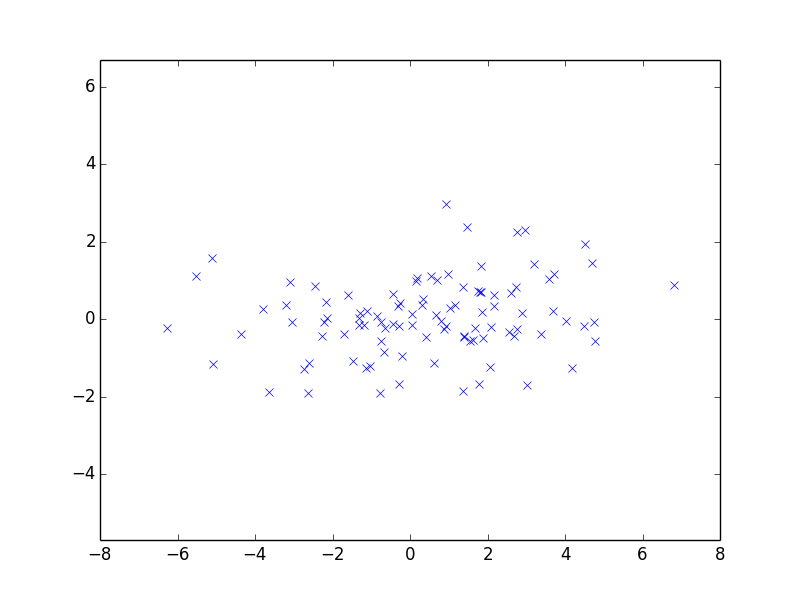
\includegraphics[width=0.9\linewidth, height=5cm]{2a} 
\caption{2a}
\label{fig:2a}
\end{subfigure}
\begin{subfigure}{0.5\textwidth}
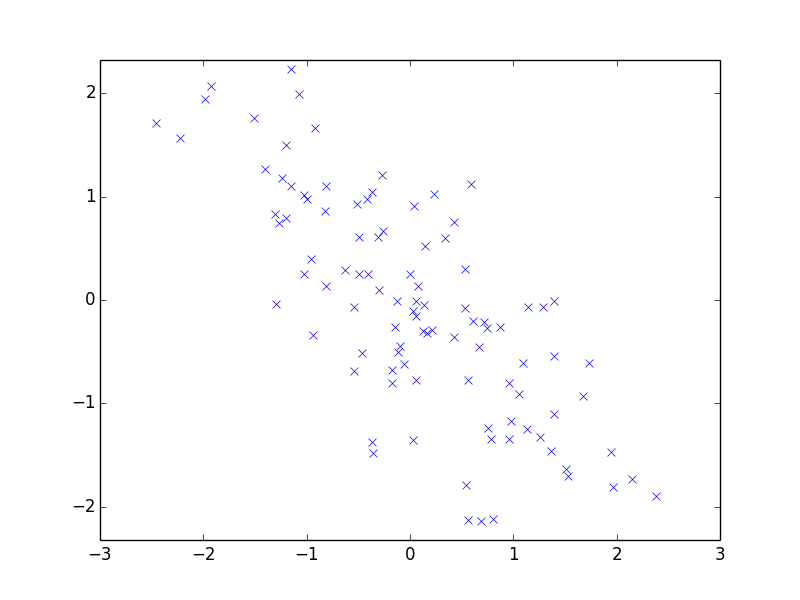
\includegraphics[width=0.9\linewidth, height=5cm]{2b}
\caption{2b}
\label{fig:2b}
\end{subfigure}
 
\caption{Bivariate Gaussian Plot}
\label{fig:plots}
\end{figure}

\section{Linear classification}
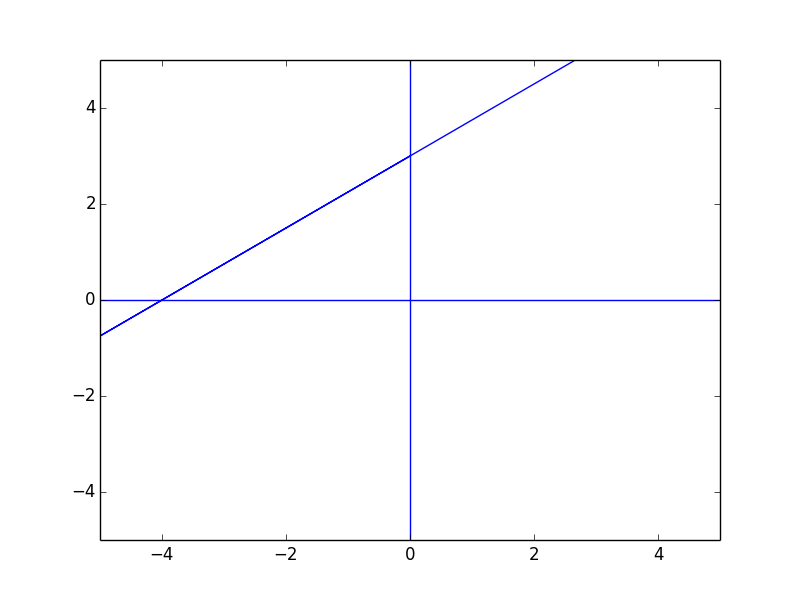
\includegraphics[width=0.5\textwidth]{3}\\
The left up side is the positive side.

\section{Eigendecomposition}
\subsection{a}
If there is no ZERO eigenvalue, then the matrix is invertible.\\
\textbf{Proof}: if $\lambda = 0$, then we have $\Sigma \cdot v = \lambda \cdot v = 0$. If $\Sigma$ is invertible, then $\Sigma \cdot v = 0$ iff $v = 0$. But according to the definition of eigenvalue, $v \neq 0$. Here is a contradiction. So if there is no zero eigenvalue, the matrix is invertible.
\subsection{b}
\[
	\Sigma \cdot v = \lambda \cdot v
\]
\begin{align*} 
	(\Sigma + c \cdot I) \cdot v & = \Sigma \cdot v + c \cdot I \cdot v \\
	& = \Sigma \cdot v + c \cdot I \cdot v \\
	& = \lambda \cdot v + c \cdot v \\
	& = (\lambda + c) \cdot v
\end{align*}
So the eigenvalues are $\lambda + c$ and the eigenvectors stay are the sane as the eigenvectors of $\Sigma$.
\subsection{c}
\begin{align*} 
	\Sigma \cdot v & = \lambda \cdot v \\
	\Sigma^{-1} \cdot \Sigma \cdot v & = \lambda \cdot \Sigma^{-1} \cdot v \\
	v & = \lambda \cdot \Sigma^{-1} \cdot v \\
	\frac{1}{\lambda} \cdot v & = \Sigma^{-1} \cdot v
\end{align*}
So the eigenvalues are $\frac{1}{\lambda}$ and the eigenvectors stay are the sane as the eigenvectors of $\Sigma$.


\section{Handwritten digit recognition using a Gaussian generative model}
\subsection{Pseudocode}

\begin{algorithm}[H]
 \KwData{train\_data, train\_label, test\_data, test\_label}
 \KwResult{parameter c which is used to smooth the covariance}
 Randomly choose 10000 number from 0 - 59999 as the validation data indexs\;
 We create the validation data and validation labels according to the indexs and the remaining as the new train data\;
 Divide the train data to 10 classes according to their labels\;
 Create the mean array and covariance matrixs for the 10 classes\;
 \For{$c$ from 0.01 to 10000}{
  Smooth the covariance by adding in $cI$\;
  Train 10 classifiers of the Gaussian generative model\;
  Apply the classifiers to the validation data to get a error rate\;
  \If{error rate is the local minimum}{
  	\Return c
   }
 }
 \caption{Pseudocode of training procedure}
\end{algorithm}

\subsection{error rate on test set}
Apply the algorithm above, we find the local minimun of error rate on validation data is when $c = 3000$.\\
Using $c = 3000$, the error rate on test data is 4.32\%
\subsection{posterior probabilities}
\noindent\begin{minipage}{0.5\textwidth}
	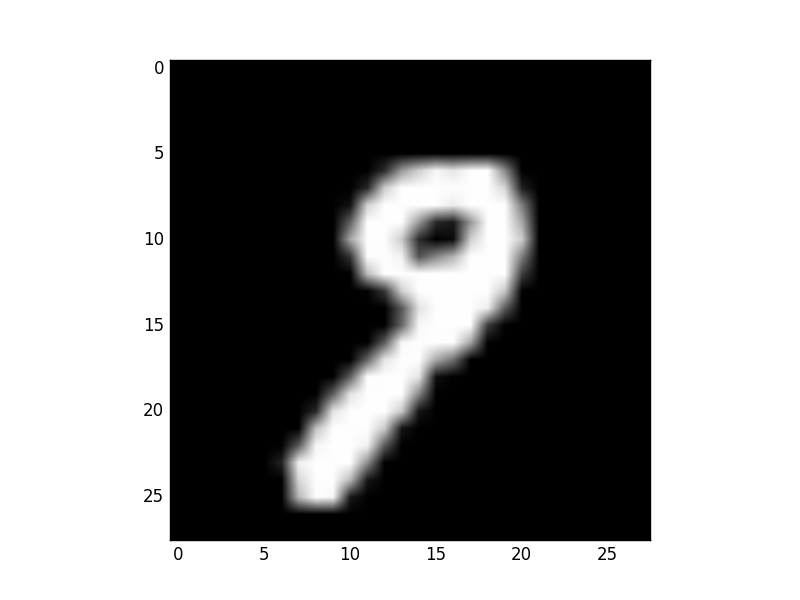
\includegraphics[width=\linewidth]{hw3_f0}
\end{minipage}%
\hfill%
\begin{minipage}{0.5\textwidth}
	Label : 9\\
	Prediction Label : 7\\
	\begin{tabular}{ | c | c | c | c | c | }
		\hline
		0 & 1 & 2 & 3 & 4 \\		
3.84e-58 &
1.88e-43 &
1.57e-34 &
8.41e-32 &
7.14e-30 \\
		\hline
		5 & 6 & 7 & 8 & 9 \\
4.91e-48 &
5.46e-89 &
0.99985 &
3.20e-14 &
0.00015 \\
		\hline
	\end{tabular}\\
\end{minipage}

\noindent\begin{minipage}{0.5\textwidth}
	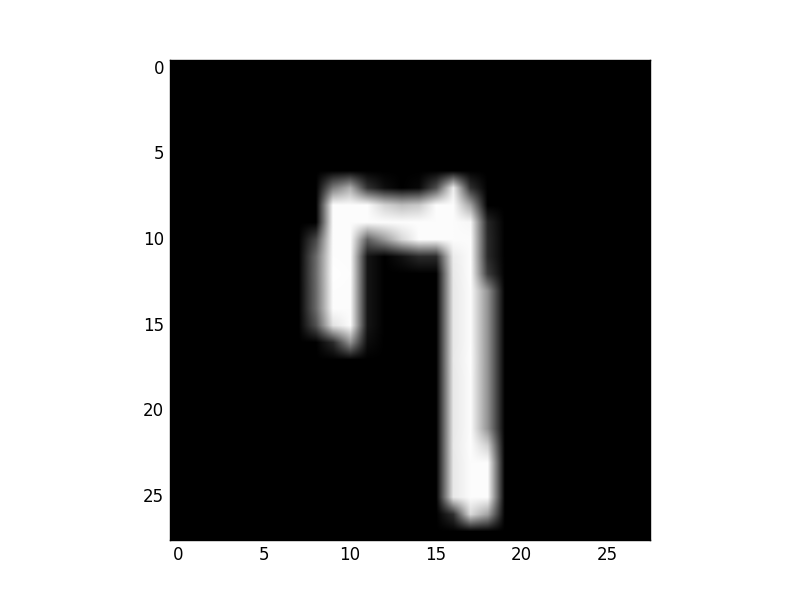
\includegraphics[width=\linewidth]{hw3_f1}
\end{minipage}%
\hfill%
\begin{minipage}{0.5\textwidth}
	Label :7\\
	Prediction Label : 9\\
	\begin{tabular}{ | c | c | c | c | c | }
		\hline
		0 & 1 & 2 & 3 & 4 \\		
5.41e-69 &
1.02e-89 &
3.53e-61 &
4.21e-42 &
8.16e-19 \\
		\hline
		5 & 6 & 7 & 8 & 9 \\
1.47e-38 &
7.94e-94 &
0.30263 &
6.97e-37 &
0.69736 \\
		\hline
	\end{tabular}\\
\end{minipage}



\noindent\begin{minipage}{0.5\textwidth}
	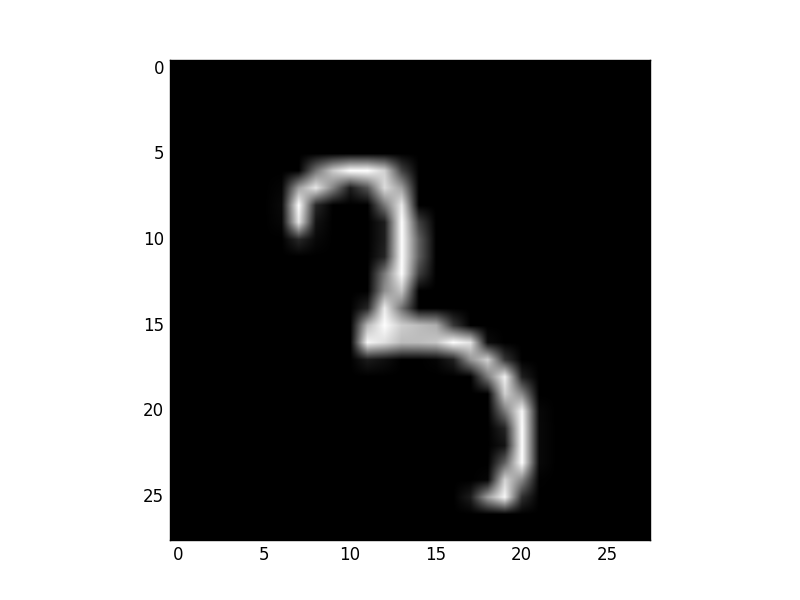
\includegraphics[width=\linewidth]{hw3_f5}
\end{minipage}%
\hfill%
\begin{minipage}{0.5\textwidth}
	Label :3\\
	Prediction Label : 4\\
	\begin{tabular}{ | c | c | c | c | c | }
		\hline
		0 & 1 & 2 & 3 & 4 \\		
3.49e-31 &
8.60e-20 &
6.15e-07 &
0.01083 &
0.71794\\
		\hline
		5 & 6 & 7 & 8 & 9 \\
0.01112 &
3.85e-22 &
6.33e-15 &
0.25865 &
0.00144 \\
		\hline
	\end{tabular}\\
\end{minipage}



\noindent\begin{minipage}{0.5\textwidth}
	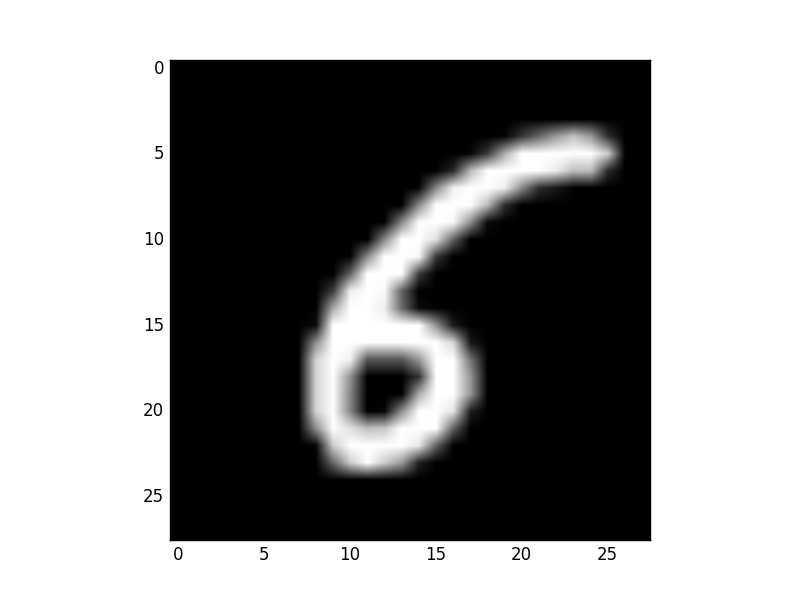
\includegraphics[width=\linewidth]{hw3_f6}
\end{minipage}%
\hfill%
\begin{minipage}{0.5\textwidth}
	Label :6\\
	Prediction Label : 5\\
	\begin{tabular}{ | c | c | c | c | c | }
		\hline
		0 & 1 & 2 & 3 & 4 \\		
2.85e-35 &
4.97e-66 &
2.76e-46 &
2.98e-35 &
7.98e-43 \\
		\hline
		5 & 6 & 7 & 8 & 9 \\
0.99999 &
4.10e-12 &
2.20e-96 &
5.35e-17 &
1.21e-75 \\
		\hline
	\end{tabular}\\
\end{minipage}



\noindent\begin{minipage}{0.5\textwidth}
	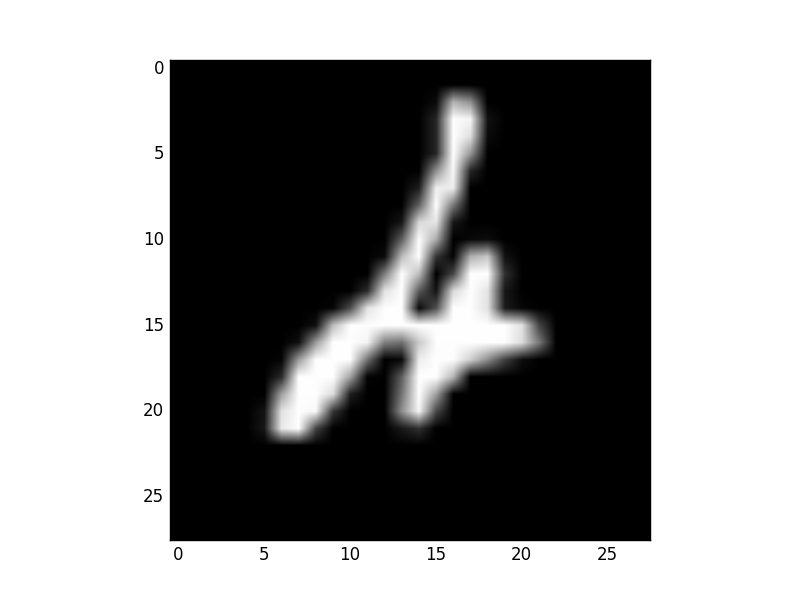
\includegraphics[width=\linewidth]{hw3_f8}
\end{minipage}%
\hfill%
\begin{minipage}{0.5\textwidth}
	Label :4\\
	Prediction Label : 6\\
	\begin{tabular}{ | c | c | c | c | c | }
		\hline
		0 & 1 & 2 & 3 & 4 \\		
7.94e-31 &
7.05e-41 &
0.00061 &
5.25e-21 &
2.04e-20 \\
		\hline
		5 & 6 & 7 & 8 & 9 \\
9.66e-25 &
0.99938 &
6.15e-53 &
4.95e-22 &
3.82e-62 \\
		\hline
	\end{tabular}\\
\end{minipage}


\section{A classifier for MNIST that occasionally abstains}
\subsection{description}
\subsection{Pseducode}
\subsection{two curves}

\end{document}




















